\documentclass[11pt,wide]{mwart}
% Kodowanie latain 2
%\usepackage[latin2]{inputenc}
\usepackage[T1]{fontenc}
% Można też użyć UTF-8
\usepackage[utf8]{inputenc}
\usepackage{listings}
\usepackage{ amssymb }
% Język
%\usepackage[polish]{babel}
% \usepackage[english]{babel}

% Rózne przydatne paczki:
% - znaczki matematyczne
%\usepackage[cp1250]{inputenc}  % Polskie literki...
\usepackage[OT4,plmath]{polski}% Polskie tytu³y, data, bibliografia, itp.
\usepackage{graphicx} 
\usepackage{amsmath, amsfonts}
% - wcięcie na początku pierwszego akapitu
\usepackage{indentfirst}
% - komenda \url w wersji nie tworzącej dodatkowej ramki
\usepackage[pdfborder={0 0 0 0}]{hyperref}
% - dołączanie obrazków
\usepackage{graphics}
\usepackage{lmodern}
% - szersza strona
\usepackage[nofoot,hdivide={2cm,*,2cm},vdivide={2cm,*,2cm}]{geometry}
\frenchspacing
% - brak numerów stron
\pagestyle{empty}
\usepackage{mathtools}
\usepackage[space]{grffile}

% dane autora
\author{Julia Majkowska}
\title{Sprawozdanie do pracowni z architektur systemów komputerowych}
\date{\today}

% początek dokumentu
\begin{document}
\maketitle

\begin{section}{Informacje o systemie}
\begin{subsection}{System operacyjny}

\begin{enumerate}
\item{Dystrybucja}  : elementary OS 0.4.1 Loki
\item{Jądro} : 143-Ubuntu SMP
\item{Wersja kompilatora} : gcc (Ubuntu 5.4.0-6ubuntu1~16.04.9) 5.4.0 


\end{enumerate}
\end{subsection}{Informacje o procesorze}
\begin{enumerate}
\item{Model}  :  Intel(R) Core(TM) i7-3740QM CPU @ 2.70GHz
\item{Pamięć Podręczna} : L1d cache:             32K,
L1i cache:             32K,
L2 cache:              256K,
L3 cache:              6144K




\end{enumerate}


\end{section}

 \begin{section}{Zadanie 1}
  \begin{subsection}{Wstęp}
  Przy mnożeniu macierzy aby policzyć wartość komórki iterujemy w jednym z czynników po wiersza a w drugim po kolumnach. Iterowanie po kolumnie dla macierzy o boku dłużyszm niż linia pamięci podręcznej wymaga ściągnięcia nowej linii przy każdej komórce tablicy. Naturale wydaje się więc zmienienie kolejnosci iterowania po macierzy, aby bardziej efektywnie wykorzystywać pamięć podręczną. 
  Innym rozwiązaniem jest zamiast liczyć od razu wartośc komórki macierzy wynikowej liczenie wartości iloczynu mniejszych minorów macierzy wejściowych. Wartość komórki macierzy jest sumą odpowiednich komórek iloczynów pewnych minorów macierzy wejściowych. Dzięki takiemu przeglądaniu danych możemy wielokrotnie korzystać jednej linii cache'a.
    W tym eksperymencie będziemy badać jak takie zmiany w kolejności wykonywanych operacji wpływają na wydajność algortymu. 
    
    
   \end{subsection}
   \begin{subsection}{Wyniki}

\begin{center}
\begin{tabular}{|c|c|c|c|c|}
\hline
Numer pomiaru, v 0 & n = 128 & n = 256 & n = 512 & n = 1024\\
\hline
0 & 0.005043 & 0.049834 & 0.201798 & 7.60244\\
\hline
1 & 0.001851 & 0.028322 & 0.220126 & 7.78302\\
\hline
2 & 0.001834 & 0.034666 & 0.226241 & 7.43234\\
\hline
3 & 0.001929 & 0.028624 & 0.215067 & 7.92553\\
\hline
4 & 0.001839 & 0.030583 & 0.34576 & 9.22362\\
\hline
5 & 0.00184 & 0.032301 & 0.207428 & 7.40595\\
\hline
6 & 0.00193 & 0.026689 & 0.215642 & 7.59781\\
\hline
7 & 0.001858 & 0.037604 & 0.251868 & 9.11708\\
\hline
8 & 0.001917 & 0.02816 & 0.217453 & 7.73221\\
\hline
9 & 0.003106 & 0.023516 & 0.236058 & 7.4264\\
\hline
SREDNIE & 0.0023147 & 0.0320299 & 0.233744 & 7.92464\\
\hline
MIN & 0.001834 & 0.023516 & 0.201798 & 7.40595\\
\hline
MAKS & 0.005043 & 0.049834 & 0.34576 & 9.22362\\
\hline
\end{tabular}
\end{center}
   
   \begin{center}
\begin{tabular}{|c|c|c|c|c|}
\hline
Numer pomiaru, v 1 & n = 128 & n = 256 & n = 512 & n = 1024\\
\hline
0 & 0.002216 & 0.020315 & 0.096102 & 0.934507\\
\hline
1 & 0.001459 & 0.011856 & 0.095804 & 1.01502\\
\hline
2 & 0.001501 & 0.012274 & 0.105682 & 0.913755\\
\hline
3 & 0.001464 & 0.011121 & 0.100786 & 1.08599\\
\hline
4 & 0.001457 & 0.012866 & 0.136235 & 1.01406\\
\hline
5 & 0.001468 & 0.013577 & 0.099623 & 0.937167\\
\hline
6 & 0.001459 & 0.01099 & 0.098083 & 1.01259\\
\hline
7 & 0.00146 & 0.014839 & 0.13078 & 0.930861\\
\hline
8 & 0.001448 & 0.011965 & 0.0949 & 1.00558\\
\hline
9 & 0.001468 & 0.011097 & 0.096032 & 0.904493\\
\hline
SREDNIE & 0.00154 & 0.01309 & 0.105403 & 0.975403\\
\hline
MIN & 0.001448 & 0.01099 & 0.0949 & 0.904493\\
\hline
MAKS & 0.002216 & 0.020315 & 0.136235 & 1.08599\\
\hline
\end{tabular}
\end{center}

\begin{center}
\begin{tabular}{|c|c|c|c|c|}
\hline
Numer pomiaru, v 2 & n = 128 & n = 256 & n = 512 & n = 1024\\
\hline
0 & 0.006737 & 0.114877 & 1.9289 & 16.8685\\
\hline
1 & 0.006842 & 0.087863 & 2.03757 & 16.4358\\
\hline
2 & 0.006831 & 0.090292 & 2.03033 & 16.2116\\
\hline
3 & 0.007036 & 0.087792 & 2.04796 & 16.2065\\
\hline
4 & 0.007363 & 0.089444 & 2.09596 & 16.9274\\
\hline
5 & 0.006847 & 0.094922 & 2.02899 & 16.6356\\
\hline
6 & 0.007239 & 0.089188 & 2.07417 & 16.8122\\
\hline
7 & 0.005807 & 0.09725 & 2.06441 & 16.002\\
\hline
8 & 0.007197 & 0.087275 & 2.08006 & 16.2529\\
\hline
9 & 0.00563 & 0.099069 & 2.05465 & 15.943\\
\hline
SREDNIE & 0.0067529 & 0.0937972 & 2.0443 & 16.4295\\
\hline
MIN & 0.00563 & 0.087275 & 1.9289 & 15.943\\
\hline
MAKS & 0.007363 & 0.114877 & 2.09596 & 16.9274\\
\hline
\end{tabular}
\end{center}

\begin{center}
\begin{tabular}{|c|c|c|c|c|}
\hline
Numer pomiaru, v 3, B= 8 & n = 128 & n = 256 & n = 512 & n = 1024\\
\hline
0 & 0.00257 & 0.02296 & 0.197326 & 1.02865\\
\hline
1 & 0.002125 & 0.015924 & 0.166596 & 1.00989\\
\hline
2 & 0.002017 & 0.015704 & 0.157289 & 1.01646\\
\hline
3 & 0.001945 & 0.015551 & 0.156243 & 1.02733\\
\hline
4 & 0.001897 & 0.023618 & 0.164099 & 1.11526\\
\hline
5 & 0.002038 & 0.019831 & 0.152751 & 1.06047\\
\hline
6 & 0.002133 & 0.027423 & 0.172617 & 1.05511\\
\hline
7 & 0.002009 & 0.027127 & 0.153678 & 0.993178\\
\hline
8 & 0.002124 & 0.016477 & 0.16059 & 1.02365\\
\hline
9 & 0.002133 & 0.018041 & 0.153027 & 1.0398\\
\hline
SREDNIE & 0.0020991 & 0.0202656 & 0.163422 & 1.03698\\
\hline
MIN & 0.001897 & 0.015551 & 0.152751 & 0.993178\\
\hline
MAKS & 0.00257 & 0.027423 & 0.197326 & 1.11526\\
\hline
\end{tabular}
\end{center}
   
 \begin{center}
 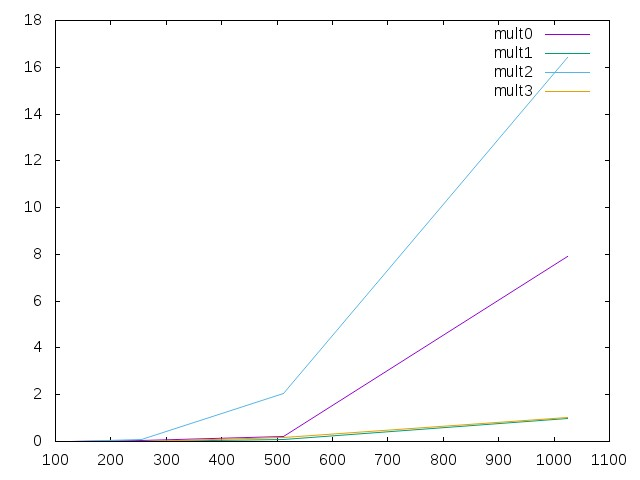
\includegraphics[scale=0.75]{wykres.jpg}
 \end{center}
 Najbardziej efektywna jest funkcja mult1 i mult3. Funkcja mult1 iteruje po kolumnach w najbardziej zewnętrznej pętli a w wewnętrznych iteruje po wierszach, a zatem wykorzystujemy więcej niż jedno słowo sprowadzonej linii cache. Funkcja mult3 wykorzystuje kafelkowanie, aby zapewnić lokalność przestrzenną. Dla obliczenia iloczynu dwóch kafelków zbiór roboczy jest na tyle mały, że mieści się w pamięci podręcznej. W funkcji mult0 iterujemy się w jednej macierzy po wierszach a w drugiej po kolumnach. Dostępy do pierwszej macierzy są sumarycznie dosyć szybkie jednak dostępy do drugiej powodują chybienie przy każdym zapytaniu. W funkcji mult2 iterujemy się w macierzy wynikowej po kolumnach i w jednej z czynnków po kolumach. Dostępy do obu z tych macierzy powodują chybienie za każdym razem, dlatego ta funkcja jest najmniej efektywna. Wyniki te są zgodne z wynikami ze slajdu. 
 \begin{center}
\begin{tabular}{|c|c|c|c|c|c|}
\hline
n = 1024 & B = 4 & B = 8 & B = 16 & B = 32 & B = 64\\
\hline
0 & 2.22952 & 1.02865 & 1.01962 & 1.22656 & 1.29741\\
\hline
1 & 1.83143 & 1.00989 & 1.06945 & 1.32835 & 1.25662\\
\hline
2 & 2.31211 & 1.01646 & 1.0979 & 1.23454 & 1.23807\\
\hline
3 & 2.47415 & 1.02733 & 1.04968 & 1.22041 & 1.30145\\
\hline
4 & 2.60534 & 1.11526 & 1.04036 & 1.2197 & 1.22903\\
\hline
5 & 2.35059 & 1.06047 & 1.05226 & 1.29735 & 1.22755\\
\hline
6 & 1.87955 & 1.05511 & 1.05211 & 1.35245 & 1.23266\\
\hline
7 & 1.99711 & 0.993178 & 1.03582 & 1.24623 & 1.21494\\
\hline
8 & 1.99886 & 1.02365 & 1.04367 & 1.33302 & 1.23487\\
\hline
9 & 2.19968 & 1.0398 & 1.07726 & 1.18746 & 1.22628\\
\hline
SREDNIE & 2.18784 & 1.03698 & 1.05381 & 1.26461 & 1.24589\\
\hline
MIN & 1.83143 & 0.993178 & 1.01962 & 1.18746 & 1.21494\\
\hline
MAKS & 2.60534 & 1.11526 & 1.0979 & 1.35245 & 1.30145\\
\hline
\end{tabular}
\end{center}
Zauważalne jest, że kafelki o rozmiarze 8 i 16 skutkują najlepszą wydajnością.
   \end{subsection}
 \end{section}

 \begin{section}{Zadanie 3}
  \begin{subsection}{Wstęp}
 	Przy wykonywaniu transpozycji metodą naiwną iterujemy się w jednej macierzy idąc wierszami a w drugiej idąc kolumnami. Jeżeli macież ma duży bok odpytywanie o kolejne elementy w tej samej kolumnie będzie wymagało sprowadzania za każdym razem nowego wiersza do pamięci podręcznej. Będziemy rozwiązywać ten problem metodą kafelkowania. Korzystając z tego, że macież transponowana to odpowiedne złożenie transpozycji minorów tej macierzy, będziemy iterować się po obu macierzach w kwadratowych blokach o niewielkiej długości boku. W ten sposób zapewnimy sobie, że aktualnie sprowadzoną linię pamięci podręcznej wykorzystamy do wyznaczenia wielu wartości macierzy transponowanej.
 
 \end{subsection}
 \begin{subsection}{Wyniki}
 
 Wykonujemy po 10 pomiarów z następującymi parametrami. Rozmiar kafelka jest zdefiniowany jako 8.
 \begin{center}
\begin{tabular}{|c|c|c|c|c|c|c|}
\hline
Numer pomiaru & -n 2048 -v 1 & -n 2048 -v 0 & -n 4096 -v 1 & -n 4096 -v 0 & -n 8192 -v 1 & -n 8192 -v 0\\
\hline
0 & 0.015907 & 0.044935 & 0.063252 & 0.186122 & 0.261985 & 0.944346\\
\hline
1 & 0.019869 & 0.05328 & 0.060263 & 0.187515 & 0.264381 & 0.91993\\
\hline
2 & 0.018595 & 0.050527 & 0.066485 & 0.183317 & 0.280471 & 1.10127\\
\hline
3 & 0.014088 & 0.041007 & 0.06894 & 0.183448 & 0.26027 & 0.902661\\
\hline
4 & 0.014494 & 0.046529 & 0.063463 & 0.196708 & 0.277106 & 1.02395\\
\hline
5 & 0.014319 & 0.041086 & 0.062603 & 0.189269 & 0.260272 & 0.927733\\
\hline
6 & 0.015409 & 0.053081 & 0.06161 & 0.192391 & 0.258154 & 1.0632\\
\hline
7 & 0.013934 & 0.040348 & 0.05987 & 0.182798 & 0.26072 & 1.04678\\
\hline
8 & 0.016072 & 0.063021 & 0.06168 & 0.20616 & 0.260446 & 1.00938\\
\hline
9 & 0.018669 & 0.067183 & 0.060153 & 0.210194 & 0.253454 & 0.893869\\
\hline
SREDNIE & 0.0161356 & 0.0500997 & 0.0628319 & 0.191792 & 0.263726 & 0.983312\\
\hline
MIN & 0.013934 & 0.040348 & 0.05987 & 0.182798 & 0.253454 & 0.893869\\
\hline
MAKS & 0.019869 & 0.067183 & 0.06894 & 0.210194 & 0.280471 & 1.10127\\
\hline
\end{tabular}
\end{center}

Kafelkowanie powoduje ok 4 krotny wzrost wydajności.

\begin{center}
\begin{tabular}{|c|c|c|c|c|c|c|}
\hline
N = 2048 & wersja naiwan & B = 4 & B = 8 & B = 16 & B = 32 & B = 64\\
\hline
0 & 0.044935 & 0.015352 & 0.015907 & 0.009829 & 0.013076 & 0.011212\\
\hline
1 & 0.05328 & 0.016087 & 0.019869 & 0.009729 & 0.009986 & 0.009938\\
\hline
2 & 0.050527 & 0.01413 & 0.018595 & 0.0109 & 0.009606 & 0.013693\\
\hline
3 & 0.041007 & 0.015411 & 0.014088 & 0.0097 & 0.014183 & 0.012666\\
\hline
4 & 0.046529 & 0.017095 & 0.014494 & 0.010403 & 0.012148 & 0.010356\\
\hline
5 & 0.041086 & 0.020156 & 0.014319 & 0.013203 & 0.014517 & 0.009756\\
\hline
6 & 0.053081 & 0.016983 & 0.015409 & 0.009977 & 0.01331 & 0.012378\\
\hline
7 & 0.040348 & 0.015451 & 0.013934 & 0.0109 & 0.008864 & 0.011667\\
\hline
8 & 0.063021 & 0.015495 & 0.016072 & 0.010715 & 0.011025 & 0.0139\\
\hline
9 & 0.067183 & 0.015815 & 0.018669 & 0.011433 & 0.008854 & 0.01041\\
\hline
SREDNIE & 0.0500997 & 0.0161975 & 0.0161356 & 0.0106789 & 0.0115569 & 0.0115976\\
\hline
MIN & 0.040348 & 0.01413 & 0.013934 & 0.0097 & 0.008854 & 0.009756\\
\hline
MAKS & 0.067183 & 0.020156 & 0.019869 & 0.013203 & 0.014517 & 0.0139\\
\hline
\end{tabular}
\end{center}

\begin{center}
\begin{tabular}{|c|c|c|c|c|c|c|}
\hline
N = 256 & wersja naiwna & B = 4 & B = 8 & B = 16 & B = 32 & B = 64\\
\hline
0 & 0.000316 & 0.000159 & 0.000172 & 0.000205 & 0.000179 & 0.000187\\
\hline
1 & 0.000252 & 0.000171 & 0.000258 & 0.000205 & 0.000175 & 0.000187\\
\hline
2 & 0.000189 & 0.00016 & 7e-05 & 0.000231 & 0.000161 & 6.8e-05\\
\hline
3 & 0.000221 & 0.000216 & 7.9e-05 & 0.00021 & 0.000161 & 8.1e-05\\
\hline
4 & 0.000217 & 0.000231 & 0.0001 & 0.000161 & 0.000152 & 6.9e-05\\
\hline
5 & 0.000198 & 0.000148 & 6.9e-05 & 0.000149 & 0.000133 & 7.7e-05\\
\hline
6 & 0.000195 & 0.000151 & 6.8e-05 & 0.00015 & 0.000156 & 6.8e-05\\
\hline
7 & 0.000209 & 0.000141 & 6.8e-05 & 0.000149 & 0.000141 & 6.8e-05\\
\hline
8 & 0.000192 & 0.000141 & 6.8e-05 & 0.000149 & 0.00014 & 6.8e-05\\
\hline
9 & 0.000189 & 0.000141 & 6.9e-05 & 0.000172 & 0.000141 & 6.8e-05\\
\hline
SREDNIE & 0.0002178 & 0.0001659 & 0.0001021 & 0.0001781 & 0.0001539 & 9.41e-05\\
\hline
MIN & 0.000189 & 0.000141 & 6.8e-05 & 0.000149 & 0.000133 & 6.8e-05\\
\hline
MAKS & 0.000316 & 0.000231 & 0.000258 & 0.000231 & 0.000179 & 0.000187\\
\hline
\end{tabular}
\end{center}


\begin{center}
\begin{tabular}{|c|c|c|c|c|c|c|}
\hline
N = 64 &wersja naiwna & B = 4 & B = 8 & B = 16 & B = 32 & B = 64\\
\hline
0 & 8e-06 & 1e-05 & 1.1e-05 & 1.2e-05 & 1.5e-05 & 1.8e-05\\
\hline
1 & 3e-06 & 1e-05 & 1.1e-05 & 1.2e-05 & 1e-05 & 1e-05\\
\hline
2 & 3e-06 & 1.4e-05 & 1.1e-05 & 1.3e-05 & 1.1e-05 & 7e-06\\
\hline
3 & 3e-06 & 1e-05 & 4e-06 & 1.7e-05 & 1e-05 & 4e-06\\
\hline
4 & 3e-06 & 9e-06 & 4e-06 & 1e-05 & 1e-05 & 4e-06\\
\hline
5 & 3e-06 & 9e-06 & 4e-06 & 1.1e-05 & 9e-06 & 4e-06\\
\hline
6 & 5e-06 & 8e-06 & 4e-06 & 9e-06 & 9e-06 & 4e-06\\
\hline
7 & 4e-06 & 9e-06 & 4e-06 & 9e-06 & 9e-06 & 4e-06\\
\hline
8 & 4e-06 & 8e-06 & 4e-06 & 1e-05 & 8e-06 & 4e-06\\
\hline
9 & 3e-06 & 8e-06 & 4e-06 & 9e-06 & 9e-06 & 4e-06\\
\hline
SREDNIE & 3.9e-06 & 9.5e-06 & 6.1e-06 & 1.12e-05 & 1e-05 & 6.3e-06\\
\hline
MIN & 3e-06 & 8e-06 & 4e-06 & 9e-06 & 8e-06 & 4e-06\\
\hline
MAKS & 8e-06 & 1.4e-05 & 1.1e-05 & 1.7e-05 & 1.5e-05 & 1.8e-05\\
\hline
\end{tabular}
\end{center}

Dla n = 64, wersja naiwna działa szybciej. Może to wynikać z tego, że przy kafelkowaniu występują dodatkowe operacje arytmetyczne na dodatkowe pętle i adresy zależące od 4 zmiennych, a oszczędność na dostępach do pamięci jest relatywnie niewielka ponieważ zbiór roboczy mieści się w L2 ( program nie dopuszcza przyjęcia mniejszego zbioru roboczego, żeby przetestować zbiór roboczy mieszczący się w L1). Dla większych n-ów, różnica wydajności rośnie wraz z n. Zbiór roboczy dla n = 256 mieści się w L2 a dla n = 1024 nie mieści się w L3. 

\end{subsection}
 
 \end{section}
 
 \begin{section}{Zadanie 4}
 
 \begin{subsection}{Wstęp}
 Przy potokowej obsłudze instrukcji, potrzebne jest przewidywanie wartości skoków. Wynika to z tego, że zanim operacja skoku zostanie zewaluowana, następne instrukcje są przetwarzane. Jeśli wartość skoku jest źle przewidziana, to należy unieważnić aktualnie rozpocząte instukcje ze złej gałęzi programu, co powoduje spadek wydajnosći. Jeżeli skoki w programie zależą od wartości losowej przewidywanie wartości skoków warunkowych jest bardzo trudne, więc czesto musimy unieważniać gałąź. 
 Aby zwiększyć wydajność redukuje liczbe skoków warunkowych, zależnych od danych losowych. Skoki zależne od wartości d zamieniłam na odwołanie do tablicy, a normalizację wartości zamieniłam na przypisanie warunkowe, które ewaluuje się do cmov.
 \end{subsection}
 
\begin{subsection}{Wyniki}

Pomiary wykonywałam dla s = 16 i t =14 i jednego ziarna losowego. 
 
\begin{center}
\begin{tabular}{|c|c|c|c|c|c|c|}
\hline
Numer pomiaru &  -n 15 -v 1 & -n 15 -v 0 & -n 10 -v 1 & -n 10 -v 0 & -n 9 -v 1 & -n 9 -v 0 \\
\hline
0 & 3.58379 & 6.48429 & 3.05228 & 6.30439 & 3.13566 & 6.39886\\
\hline
1 & 3.57743 & 6.53884 & 3.10654 & 6.36823 & 3.0384 & 6.24283\\
\hline
2 & 3.59665 & 6.28596 & 3.0329 & 6.31317 & 3.0257 & 6.55421\\
\hline
3 & 3.59451 & 6.41994 & 3.0378 & 6.22986 & 3.03 & 6.51263\\
\hline
4 & 3.55936 & 6.34573 & 3.1784 & 6.33898 & 3.09568 & 6.226\\
\hline
5 & 3.56534 & 6.36005 & 3.07649 & 6.38996 & 3.14208 & 6.47716\\
\hline
6 & 3.58768 & 6.46088 & 3.02789 & 6.45783 & 3.1428 & 6.30613\\
\hline
7 & 3.70552 & 6.36446 & 3.30739 & 6.35524 & 3.03566 & 6.2263\\
\hline
8 & 3.60102 & 6.27782 & 3.1775 & 6.6928 & 3.17718 & 6.28077\\
\hline
9 & 3.56645 & 6.36821 & 3.22907 & 6.44435 & 3.0741 & 6.18908\\
\hline
SREDNIE & 3.59377 & 6.39062 & 3.12263 & 6.38948 & 3.08973 & 6.3414\\
\hline
MIN & 3.55936 & 6.27782 & 3.02789 & 6.22986 & 3.0257 & 6.18908\\
\hline
MAKS & 3.70552 & 6.53884 & 3.30739 & 6.6928 & 3.17718 & 6.55421\\
\hline
\end{tabular}
\end{center}


\begin{center}
\begin{tabular}{|c|c|c|c|c|}
\hline
Numer pomiaru &  -n 8 -v 1 & -n 8 -v 0 & -n 7 -v 1 & -n 7 -v 0 \\
\hline
0 & 3.04674 & 6.22644 & 3.0451 & 6.32677\\
\hline
1 & 3.22712 & 6.52771 & 3.15923 & 6.35592\\
\hline
2 & 3.24865 & 6.31952 & 3.02855 & 6.26207\\
\hline
3 & 3.11274 & 6.21531 & 3.04584 & 6.23032\\
\hline
4 & 3.03211 & 6.26246 & 3.01516 & 6.39234\\
\hline
5 & 3.31139 & 6.49374 & 3.01073 & 6.2917\\
\hline
6 & 3.1204 & 6.3635 & 3.13134 & 6.4151\\
\hline
7 & 3.03946 & 6.26719 & 3.13011 & 6.23858\\
\hline
8 & 3.0527 & 6.19953 & 3.06648 & 6.19986\\
\hline
9 & 3.0179 & 6.22511 & 3.02245 & 6.25194\\
\hline
SREDNIE & 3.12092 & 6.31005 & 3.0655 & 6.29646\\
\hline
MIN & 3.0179 & 6.19953 & 3.01073 & 6.19986\\
\hline
MAKS & 3.31139 & 6.52771 & 3.15923 & 6.4151\\
\hline
\end{tabular}
\end{center}
Zauważamy ok. 2 krotne przyspieszenie dla każdego n. Dodatkowo dla n = 15 wersja przyspieszona działa zauważalnie wolniej niż dla mniejszych n-ów, pomimo takiej samej liczby wykonanych kroków. Wynika to, że taki obszar roboczy nie mieści się w cache'u L1, a dla mniejszych n-ów się mieści.
\end{subsection}

\end{section}


 
 \begin{section}{Zadanie 5}
 
 \begin{subsection}{Wstęp}
 	Wyszukiwanie binarne charakteryzuje się niską lokalnością w początkowej fazie wyszukiwania. Z każdą iteracją odległość końców przedziałów wyszukiwania zmniejsza się dwukrotnie i na początku jest równa liczbie n elementów w ciągu. Zatem dla odpowiednio dużego n i początkowych iteracji sprowadzamy do pamięci podręcznej nowy wiersz. Dodatkowo to, który wiersz sprowadzimy zależy od wyniku porównania, a zatem jest trudny przewidzenia. 
 	
 	Jeżeli zorganizujemy dane w porządku kopcowym w tablicy, początkowe zapytania będą bardzo zbliżone w pamięci i pierwsze 2 - 3 poziomy drzewa zmieszczą się w jednym wierszu pamięci podręcznej. Ponadto, dwaj bracia w drzewie znajdują się w sąsiadujących komórkach pamięci, więc niezaleźnie od wyniku porównania sprowadzany jest ten sam wiersz. 
 
 \end{subsection}
 
 \begin{subsection}{Wyniki}
 
 Przeprowadziłam eksperyment dla 3 różnych rozmiarów obszarów roboczych : \( 2^ {23} , 2^{20}, 2^{15}\) słów. Przy każdym uruchomieniu wykonując \(2^{24}\) zapytań. Dla każdego rozmiaru wykonałam 10 pomiarów dla obu wersji programu i dwóch różnych ziaren losowych : 0x27841496381ef019 ,0x5bab3de5da7882ff.
 
\begin{center}
\begin{tabular}{|c|c|c|c|c|c|c|c|c|}
\hline
Numer pomiaru & -n 23 -t 24 -v 0 & -n 23 -t 24 -v 1 & -n 23 -t 24 -v 0 & -n 23 -t 24 -v 1\\
\hline
0 & 12.3054 & 3.24159 & 12.7919 & 3.43522\\
\hline
1 & 11.8219 & 3.46942 & 11.8971 & 3.37872\\
\hline
2 & 12.7894 & 3.25246 & 12.4521 & 3.55149\\
\hline
3 & 11.794 & 3.19846 & 11.784 & 3.29874\\
\hline
4 & 13.1803 & 3.52636 & 11.7435 & 3.56357\\
\hline
5 & 12.6183 & 3.26543 & 12.516 & 3.33372\\
\hline
6 & 12.5433 & 3.24456 & 11.8782 & 3.5116\\
\hline
7 & 11.492 & 3.44676 & 11.7512 & 3.1635\\
\hline
8 & 12.7275 & 3.70262 & 12.5029 & 3.42147\\
\hline
9 & 13.0012 & 3.43737 & 12.1751 & 3.28438\\
\hline
SREDNIE & 12.4273 & 3.3785 & 12.1492 & 3.39424\\
\hline
MIN & 11.492 & 3.19846 & 11.7435 & 3.1635\\
\hline
MAKS & 13.1803 & 3.70262 & 12.7919 & 3.56357\\
\hline
\end{tabular}
\end{center}

Wydać zauważalną różnicę w wydajności. Eksperyment dla wariantu kopcowego trwał \(27.1\%\) i \(27.9\%\) czasu eksperymentu dla wariantu ze zwykłym wyszukiwaniem binarnym. \\


\begin{center}
\begin{tabular}{|c|c|c|c|c|}
\hline
Numer pomiaru & -n 20 -t 24 -v 0 & -n 20 -t 24 -v 1 & -n 20 -t 24 -v 0 & -n 20 -t 24 -v 1\\
\hline
0 & 2.66699 & 1.51926 & 2.61153 & 1.52456\\
\hline
1 & 2.60155 & 1.55698 & 2.62126 & 1.60389\\
\hline
2 & 2.68956 & 1.5442 & 2.66771 & 1.58656\\
\hline
3 & 2.66278 & 1.6018 & 2.63655 & 1.53997\\
\hline
4 & 2.71261 & 1.5263 & 2.61501 & 1.51517\\
\hline
5 & 3.20788 & 1.84454 & 3.19343 & 1.53553\\
\hline
6 & 2.65966 & 1.57196 & 2.73109 & 1.62111\\
\hline
7 & 2.54166 & 1.51098 & 2.54854 & 1.51634\\
\hline
8 & 4.12462 & 1.85509 & 4.27662 & 1.83477\\
\hline
9 & 2.6734 & 1.54089 & 2.62791 & 1.51343\\
\hline
SREDNIE & 2.85407 & 1.6072 & 2.85296 & 1.57913\\
\hline
MIN & 2.54166 & 1.51098 & 2.54854 & 1.51343\\
\hline
MAKS & 4.12462 & 1.85509 & 4.27662 & 1.83477\\
\hline
\end{tabular}
\end{center}

Różnica wydajności jest mniej zauważalna, wariant kopcowy działa około 2-krotnie szybciej niż wariant z wyszukiwaniem binarnym.



\begin{center}
\begin{tabular}{|c|c|c|c|c|}
\hline
Numer pomiaru & -n 15 -t 24 -v 0 & -n 15 -t 24 -v 1 & -n 15 -t 24 -v 0 & -n 15 -t 24 -v 1\\
\hline
0 & 0.765121 & 0.685628 & 0.739127 & 0.729057\\
\hline
1 & 0.756895 & 0.683885 & 0.773129 & 0.68564\\
\hline
2 & 0.737829 & 0.713604 & 0.692509 & 0.707761\\
\hline
3 & 0.714133 & 0.673465 & 0.732179 & 0.667067\\
\hline
4 & 0.732084 & 0.670414 & 0.744528 & 0.667337\\
\hline
5 & 0.738551 & 0.690977 & 0.733958 & 0.698666\\
\hline
6 & 0.73628 & 0.688645 & 0.725323 & 0.687195\\
\hline
7 & 0.723849 & 0.666851 & 0.771843 & 0.676446\\
\hline
8 & 0.723121 & 0.658983 & 0.717397 & 0.67681\\
\hline
9 & 0.721841 & 0.70823 & 0.694926 & 0.729827\\
\hline
SREDNIE & 0.73497 & 0.684068 & 0.732492 & 0.692581\\
\hline
MIN & 0.714133 & 0.658983 & 0.692509 & 0.667067\\
\hline
MAKS & 0.765121 & 0.713604 & 0.773129 & 0.729827\\
\hline
\end{tabular}
\end{center}


Wariant kopcowy nieznacznie szybciej niż wariant z wyszukiwaniem bianrnym. Zbiór roboczy jest na tyle mały,  że mieści się w pamięci podręcznej L3, zatem przy wielu zapytaniach czas chybień w pamięć podręczną staje się mniej istotną częścią czasu wykonywania. 

Bez zmiany działania można zamienić miejscami dwie instrukcje warunkowe w ciele pętli. Nie powoduje to jednak przyspieszenia. Przed zamianą instrukcja
\begin{lstlisting}
 if (y \< x) j |= 1; 
 \end{lstlisting}jest zamieniana przez kompilator na instrukcję
 \begin{lstlisting}
  cmovl  \%r8,\%rax
  \end{lstlisting}, a po zamianie na skok warunkowy, który może generować dodatkowe koszty przy pomyłce w przewidywaniu skoków. 

\end{subsection}
\end{section}
\begin{section}{Zadanie 6}
\begin{subsection}{Rozmiar linii cache}
Będziemy przeszukiwać kolejne elementy tablicy oddalone od siebie o j. Jeżeli długość skoku będzie krótsza niż długość linii to będziemy odczytywać więcej niż jedną wartość z danej linii a zatem wydajność będzie lepsza. Jeżeli długość skoku będzie większa niż długość linii to chybienia będą następować przy każdym zapytaniu. Rozmiar zbioru roboczego przyjęłam \(2^{16}\), aby mieścił się w cache'u L2 i koszt chybienia był w miarę jednolity. Liczba kroków to \(2^{16}\).
\begin{center}
\begin{tabular}{|c|c|}
\hline
j - dlugosc skoku & wynik sredniego pomiaru \\
\hline
4 & 0.164729\\
\hline
8 & 0.162257\\
\hline
12 & 0.192912\\
\hline
16 & 0.277085\\
\hline
20 & 0.295606\\
\hline
24 & 0.292245\\
\hline
28 & 0.301763\\
\hline
32 & 0.318895\\
\hline
36 & 0.347964\\
\hline
64 & 0.364643\\
\hline
128 & 0.367078\\
\hline
256 & 0.382651\\
\hline
512 & 0.493697\\
\hline
1024 & 0.497247\\
\hline
\end{tabular}
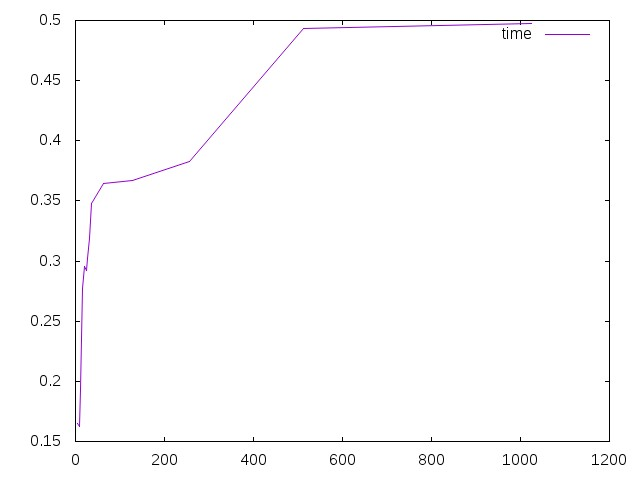
\includegraphics[scale=0.75]{wykres6a.jpg}
\end{center}

Zauważalny jest skok wartości dla skoku o 16 elementów. Wtedy odpytywanie powoduje chybienie za każdym razem. To prowadzi do wniosku, że długość linii cache to \(4*16 = 64\) B.

\end{subsection}

\begin{subsection}{Rozmiar L1, L2, L3}
W tym zadaniu będziemy szukać rozmiaru zbioru roboczego dla którego istotnie zmienia się wydajność programu. Będziemy skakać co 16 elementów, w tablicy, aby generować chybienie za każdym razem. Dla kolejnych rozmiarów zbioru roboczego będziemy mierzyć czas przejścia przez tablicę. Dla poszczególnych pierwszego zbioru roboczego przekraczającego rozmiar pamięci podręcznej powinniśmy zaobserwować znaczący spadek efektywności, spowodowany wzrostem kosztu chybień w pamięć. Liczba kroków to \(2^{16}\). 
\begin{center}
\begin{tabular}{|c|c|}
\hline
n & wynik sredniego pomiaru \\
\hline
1 & 0.499194\\
\hline
2 & 0.564769\\
\hline
3 & 0.566598\\
\hline
4 & 0.563949\\
\hline
5 & 0.559764\\
\hline
6 & 0.551561\\
\hline
7 & 0.563478\\
\hline
8 & 0.558177\\
\hline
9 & 0.544814\\
\hline
10 & 0.558845\\
\hline
11 & 0.553309\\
\hline
12 & 0.543123\\
\hline
13 & 0.545067\\
\hline
14 & 0.857375\\
\hline
15 & 0.835617\\
\hline
16 & 0.888066\\
\hline
17 & 0.956992\\
\hline
18 & 0.960283\\
\hline
19 & 0.956232\\
\hline
20 & 1.00117\\
\hline
21 & 1.15819\\
\hline
22 & 1.20874\\
\hline
23 & 1.23378\\
\hline
24 & 1.19415\\
\hline
25 & 1.17526\\
\hline
\end{tabular}

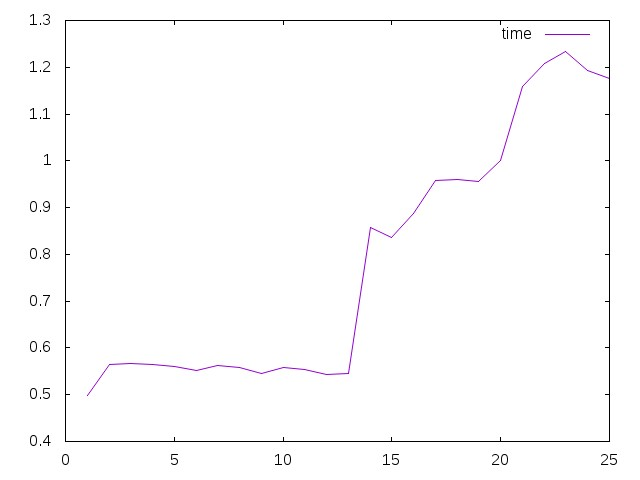
\includegraphics[scale=0.75]{wykres6b.jpg}
\end{center}

Zauważamy isotne wzrost w czasie wykonania dla n = 14, n = 17, n = 21. To prowadzi do wniosków
\begin{equation*}
L1 = 2^{13 + 2} B = 2^5 KB = 32 KB
\end{equation*}

\begin{equation*}
L2 = 2^{16 + 2} B = 2^8 KB = 256 KB
\end{equation*}

\begin{equation*}
L3 = 2^{21 + 2} B = 2^{13} KB = 8192 KB
\end{equation*}

Wyniki te są zgodne z faktycznymi pomiarami systemu z wyjątkiem L3, który ma rozmiar 6144K.Z racji, że rozmiar nie jest potegą dwójki, nie wykryłam go dokładnie, jednak wynik eksperymentu jest wielkością tego samego rzędu.
\end{subsection}
\end{section}



\end{document}
